% This file was created with matplot2tikz v0.5.3.
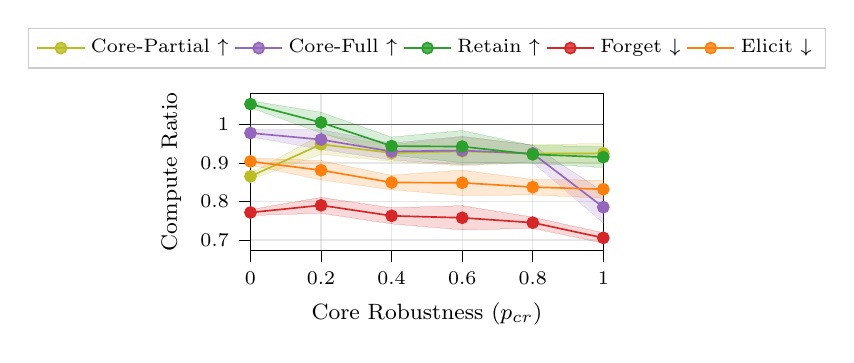
\begin{tikzpicture}

\definecolor{crimson2143940}{RGB}{214,39,40}
\definecolor{darkgray176}{RGB}{176,176,176}
\definecolor{darkorange25512714}{RGB}{255,127,14}
\definecolor{darkslategray77}{RGB}{77,77,77}
\definecolor{forestgreen4416044}{RGB}{44,160,44}
\definecolor{goldenrod18818934}{RGB}{188,189,34}
\definecolor{lightgray204}{RGB}{204,204,204}
\definecolor{mediumpurple148103189}{RGB}{148,103,189}

\begin{axis}[
label style={font=\footnotesize},
tick label style={font=\scriptsize},
title style={font=\footnotesize},
height=3.57cm,
legend cell align={left},
legend columns=5,
legend style={
  font=\scriptsize,
  fill opacity=0.8,
  draw opacity=1,
  text opacity=1,
  at={(0.5,1.16)},
  anchor=south,
  draw=lightgray204
},
tick align=outside,
tick pos=left,
width=0.5\linewidth,
x grid style={darkgray176, opacity=0.3},
xlabel={Core Robustness (\(\displaystyle p_{cr}\))},
xmajorgrids,
xmin=0, xmax=5,
xtick style={color=black},
xtick={0,1,2,3,4,5},
xticklabels={0,0.2,0.4,0.6,0.8,1},
y grid style={darkgray176, opacity=0.3},
ylabel={Compute Ratio},
ymajorgrids,
ymin=0.673541643732381, ymax=1.08066738528882,
ytick style={color=black}
]
\path [draw=goldenrod18818934, fill=goldenrod18818934, opacity=0.18, line width=0pt]
(axis cs:0,0.873116270188678)
--(axis cs:0,0.857844490080138)
--(axis cs:1,0.923073972398174)
--(axis cs:2,0.904555999072229)
--(axis cs:3,0.892874178134876)
--(axis cs:4,0.902143013099316)
--(axis cs:5,0.899379079207784)
--(axis cs:5,0.950781002896733)
--(axis cs:5,0.950781002896733)
--(axis cs:4,0.947584539528395)
--(axis cs:3,0.967717509777944)
--(axis cs:2,0.947840873129645)
--(axis cs:1,0.97448541620332)
--(axis cs:0,0.873116270188678)
--cycle;

\path [draw=mediumpurple148103189, fill=mediumpurple148103189, opacity=0.18, line width=0pt]
(axis cs:0,0.987321055138536)
--(axis cs:0,0.968871664092531)
--(axis cs:1,0.935760654508155)
--(axis cs:2,0.908293060920301)
--(axis cs:3,0.89544041549291)
--(axis cs:4,0.902273004735759)
--(axis cs:5,0.745112761850905)
--(axis cs:5,0.825308630607411)
--(axis cs:5,0.825308630607411)
--(axis cs:4,0.947007682842655)
--(axis cs:3,0.969578446394525)
--(axis cs:2,0.951946117495623)
--(axis cs:1,0.986462946220595)
--(axis cs:0,0.987321055138536)
--cycle;

\path [draw=forestgreen4416044, fill=forestgreen4416044, opacity=0.18, line width=0pt]
(axis cs:0,1.06216166976352)
--(axis cs:0,1.04448377052018)
--(axis cs:1,0.978670459922949)
--(axis cs:2,0.920825404524627)
--(axis cs:3,0.901258112171169)
--(axis cs:4,0.899374260217656)
--(axis cs:5,0.888357656378789)
--(axis cs:5,0.942529909965103)
--(axis cs:5,0.942529909965103)
--(axis cs:4,0.945722811105054)
--(axis cs:3,0.984543621660111)
--(axis cs:2,0.967606435570888)
--(axis cs:1,1.03232712763391)
--(axis cs:0,1.06216166976352)
--cycle;

\path [draw=crimson2143940, fill=crimson2143940, opacity=0.18, line width=0pt]
(axis cs:0,0.779199729764511)
--(axis cs:0,0.763707029548179)
--(axis cs:1,0.769547984305231)
--(axis cs:2,0.742011085214635)
--(axis cs:3,0.726277669640135)
--(axis cs:4,0.730514915526055)
--(axis cs:5,0.692047359257674)
--(axis cs:5,0.718856620123125)
--(axis cs:5,0.718856620123125)
--(axis cs:4,0.759493062662159)
--(axis cs:3,0.789069201996383)
--(axis cs:2,0.783554179383765)
--(axis cs:1,0.810726650507246)
--(axis cs:0,0.779199729764511)
--cycle;

\path [draw=darkorange25512714, fill=darkorange25512714, opacity=0.18, line width=0pt]
(axis cs:0,0.91350733796087)
--(axis cs:0,0.894921583751458)
--(axis cs:1,0.856464545063614)
--(axis cs:2,0.830626286409983)
--(axis cs:3,0.815748362760845)
--(axis cs:4,0.817440900546089)
--(axis cs:5,0.808735350199541)
--(axis cs:5,0.855122683874913)
--(axis cs:5,0.855122683874913)
--(axis cs:4,0.857470036325594)
--(axis cs:3,0.881548032959044)
--(axis cs:2,0.868265525502841)
--(axis cs:1,0.906140063469389)
--(axis cs:0,0.91350733796087)
--cycle;

\addplot [line width=0.32pt, darkslategray77, opacity=0.85, forget plot]
table {%
0 1
5 1
};
\addplot [semithick, goldenrod18818934, mark=*, mark size=2, mark options={solid}]
table {%
0 0.865480380134408
1 0.948779694300747
2 0.926198436100937
3 0.93029584395641
4 0.924863776313856
5 0.925080041052258
};
\addlegendentry{Core-Partial $\uparrow$}
\addplot [semithick, mediumpurple148103189, mark=*, mark size=2, mark options={solid}]
table {%
0 0.978096359615534
1 0.961111800364375
2 0.930119589207962
3 0.932509430943718
4 0.924640343789207
5 0.785210696229158
};
\addlegendentry{Core-Full $\uparrow$}
\addplot [semithick, forestgreen4416044, mark=*, mark size=2, mark options={solid}]
table {%
0 1.05332272014185
1 1.00549879377843
2 0.944215920047757
3 0.94290086691564
4 0.922548535661355
5 0.915443783171946
};
\addlegendentry{Retain $\uparrow$}
\addplot [semithick, crimson2143940, mark=*, mark size=2, mark options={solid}]
table {%
0 0.771453379656345
1 0.790137317406239
2 0.7627826322992
3 0.757673435818259
4 0.745003989094107
5 0.705451989690399
};
\addlegendentry{Forget $\downarrow$}
\addplot [semithick, darkorange25512714, mark=*, mark size=2, mark options={solid}]
table {%
0 0.904214460856164
1 0.881302304266502
2 0.849445905956412
3 0.848648197859944
4 0.837455468435842
5 0.831929017037227
};
\addlegendentry{Elicit $\downarrow$}
\end{axis}

\end{tikzpicture}
